\section{The A3-E Model}\label{sec:proposal}

\section{The Cloud-Edge-Mobile Continuum}\label{sec:continuum}

Together, the computational resources from mobile, edge, and cloud computing have the potential of forming a \textit{continuum} on which new and disruptive types of applications can rely (Fig.~\ref{fig:continuum-overral}). Sometimes referred to as the Cloud-to-Things continuum, it enables the seamless convergence of infrastructure stretching from the cloud datacenter to devices on the network edge (including intermediate devices like ISP gateways, cellular base stations, and private cloud deployments) into a continuum of resources, to be provisioned to multiple tenants for hosting applications. Components of an application are hence able to run in a geo-distributed fashion using the services provided by the distributed infrastructure~\cite{GuptaIfogSim17}. 

\subsection{Cloud}

The Cloud infrastructure is typically offered through different virtualization techniques and degrees~\cite{leitner2016patterns, Quatrocchi2016discrete}. It is considered to be a black box: this means that application developers do not have access to the hypervisor or to the underlying physical machines, which are managed by cloud providers. A Cloud instance or \textit{node} is traditionally materialized as a Virtual Machine (VM). However, nowadays a node might also be a container. Containers provide yet another virtualization technique that operates at the Operating System (OS) level, to create isolated views of the operating environment for different applications. A container has its own process space, virtualized network interface, and file system; and the operating system can allocate different amounts of resources (e.g., CPU, memory, and I/O) to each of them.

Multiple VMs are managed by a single hypervisor that resides on a single host operating system. Each VM then contains its own guest operating system, its own platform stack composed of different libraries, middleware, and application servers, and its own application code. On the other hand, containers are executed directly on top of the host operating system, optionally with the help of a container manager like Docker\footnote{Docker -- \url{http://docker.com}}. Each container has its own platform stack and its own application code. Containers have various advantages when compared to VMs: they are more lightweight and they are faster to boot and terminate because they do not have to deal with a guest
operating system~\cite{FelterContainerVm15,SoletzContainerVirt14}.
%Industry is widely adopting containers as a means to favor portability and they are considered to be one of the main technological enablers of the DevOps movement [36]. Different development teams may use different operating systems and different platform stacks, making feature integration hard. However, thanks to containerization technology, features can be developed in isolation, with the guarantee that they will work the exact same way on any machine that supports containers.

\subsection{Edge}

Edge computing can be defined by the set of technologies that enable computation to be performed at the network edge~\cite{Shi:2016}. Its main goal is to allow data produced and consumed at the network edge to be processed with low-latency and without overstressing the more centralized cloud infrastructure.

As examples of edge technologies, Cloudlets~\cite{Satyanarayanan:2009} have been first presented as mobile cloud servers that can be positioned at strategic locations to provide computing resources to resource constrained devices with low-latency. 
%with expected high density of users (e.g., at concert halls, stadiums) or areas with temporary infrastructure limitations (e.g., after disasters). 
Additionally, Mobile Edge Computing (MEC)~\cite{ahmed2016isco} relies on cellular infrastructure to enable a low-latency communication between user equipment (i.e., mobile devices) and servers. 

The main motivation for shifting computation from cloud to the network edge is the mitigation of network latency~\cite{Bonomi2014}. In specific, real-time applications are the main candidates for benefiting of services deployed at nearby edge infrastructure. For example, Augmented Reality (AR) is a type of application that would benefit from the low-latency of edge services~\cite{hu2015mobile,GarrigaMendonca2017}. Moreover, mobile devices exhibit limitations that may further motivate the use of edge computing as part of a continuum: some mobile applications rely on heavyweight tasks that can overstress the platform and limit the concurrent execution of other applications; and the battery is a valuable resource that may be significantly affected by the kind of task performed locally, as networking tends to consume less than CPU(s)~\cite{Carroll:2010}. 

\subsection{Mobile}



\subsection{Definition}

%Fig.~\ref{fig:continuum} describes the different parts of the continuum. Cloud computing features virtually unlimited computational resources and shall remain as the source of services with higher availability. Edge computing, in turn, features low network latency and shall provide services for real-time and delay-sensitive applications. Finally, despite the improvements in the capabilities of mobile devices, the later still suffer from battery drain and other platform/hardware limitations which motivates computation offloading. In addition to the commonly employed mobile-cloud inter-operation, mobile devices can integrate the continuum as both clients of computation that may opportunistically be offloaded to edge servers and providers of their own local services to cope with the situations in which edge is not available. 
%
%\begin{figure}[tbp]
%	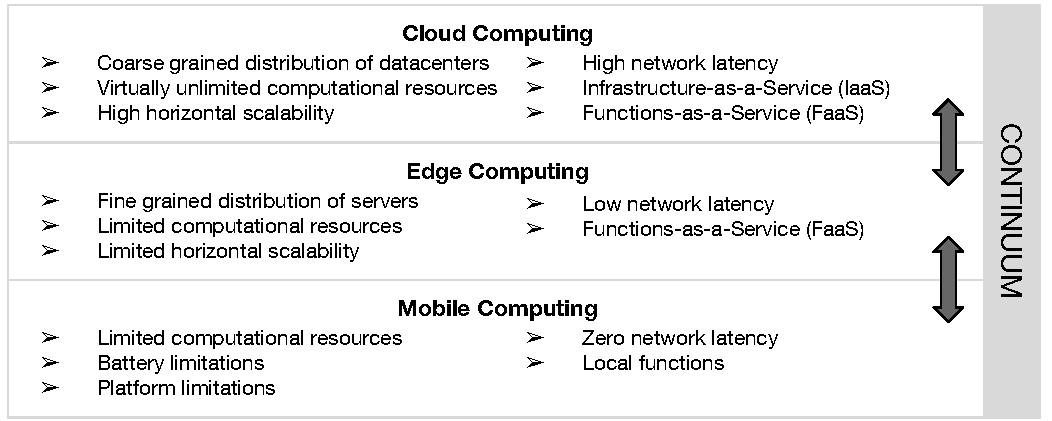
\includegraphics[width=0.9\textwidth]{figs/Continuum.pdf}
%	\caption{Computational continuum formed by Cloud, Edge, and Mobile Computing}
%	\label{fig:continuum}
%\end{figure}


\begin{figure}[tbp]
	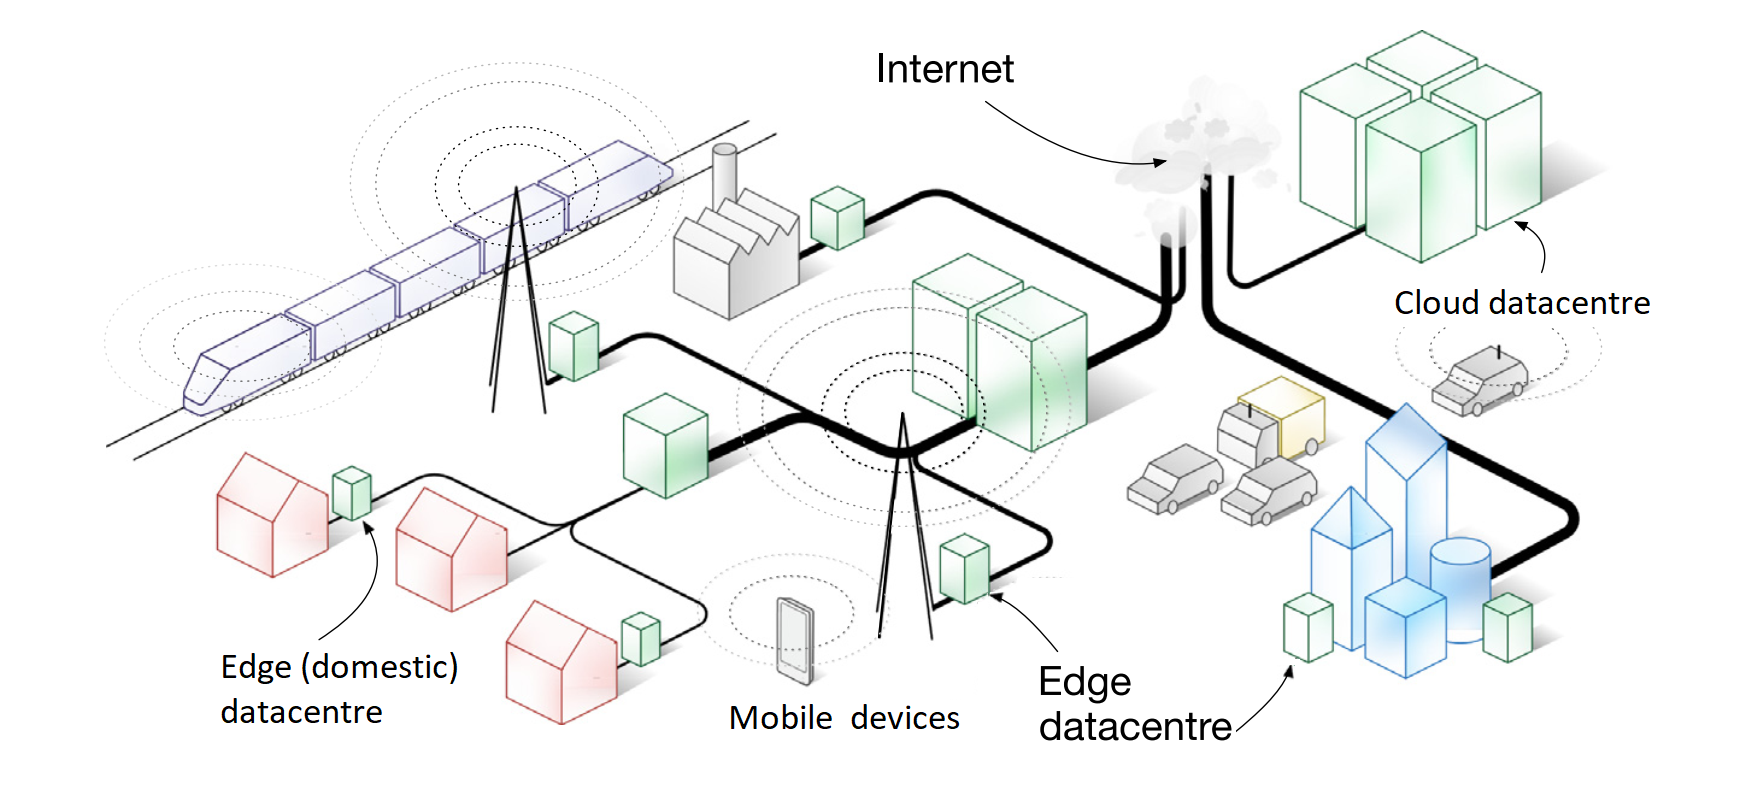
\includegraphics[width=0.9\textwidth]{figs/Continuum-overall.png}
	\caption{The computational continuum formed by coarsely distributed cloud datacenters, finely distributed edge datacenters, and mobile/IoT devices (adapted from~\cite{Tarneberg2017}).}
	\label{fig:continuum-overral}
\end{figure}

\newcounter{req_count}
\newcounter{req_sub_count}[req_count]


%TODO: parts of this paragraph are unclear (e.g., interplay with the cloud properties?)
%The key notion to bridge the gap in such a continuum is that of edge\footnote{In the literature the term ``edge'' is often used interchangeably with the term ``fog''.} computing, whose defining characteristics are edge location, dense geographical distribution, large-scale of deployment, support for mobility, resource and interface heterogeneity, and interplay with the cloud properties in order to address requirements of mobile applications that need low latency with a wide and dense geographical distribution~\cite{Bonomi2014}.  


%What: the challenges in materializing the continuum
\subsection{Key Characteristics and Challenges}

%\stepcounter{req_count}

The continuum encompasses heterogeneous types of computing platforms and technologies located at the cloud and at the edge of the network, as well as in mobile devices. Among others, the heterogeneity includes the granularity in which edge datacenters are geographically distributed, posing the challenges of efficiency and scalability of the later; it also includes the way edge services are discovered and accessed, which poses the challenge of awareness. Finally, it includes the particular constraints of mobile devices in terms of battery, platform, and hardware limitations, which adds to the factors that must be taken into account in the decision of where computation should be placed along the continuum in different contexts of operation.

%Next, we identify the key characteristics of the cloud-edge-mobile continuum posing challenges to its realization along with the properties required to address these challenges.

%This heterogeneity poses challenges in terms of how each part of the continuum should allocate its resources to different types of client applications (provisioning) and how these applications should have access to the continuum resources (inter-operation). 

%In particular, 


%The realization of the continuum requires a flexible model that copes with this heterogeneity (Req. \stepcounter{req_sub_count}\textbf{R\arabic{req_count}.\arabic{req_sub_count}}).%, i.e., different instances of the model should address the many particularities in the continuum .
%, i.e., it should be agnostic with respect to the capabilities and specific technology details of different computing platforms and infrastructures in the continuum (Req. \stepcounter{req_sub_count}\textbf{R\arabic{req_count}.\arabic{req_sub_count}}); and 


%\begin{figure}[tbp]
%	\centering
%	\captionsetup[subfigure]{width=0.51\textwidth}	
%	\null\hfill
%	\subfloat[Heterogeneus and independent types of computing platforms and infrastructure (mobile-edge, local-edge, cloud) in range of communication with a mobile device\label{fig:edge-heterogeneity}]{ 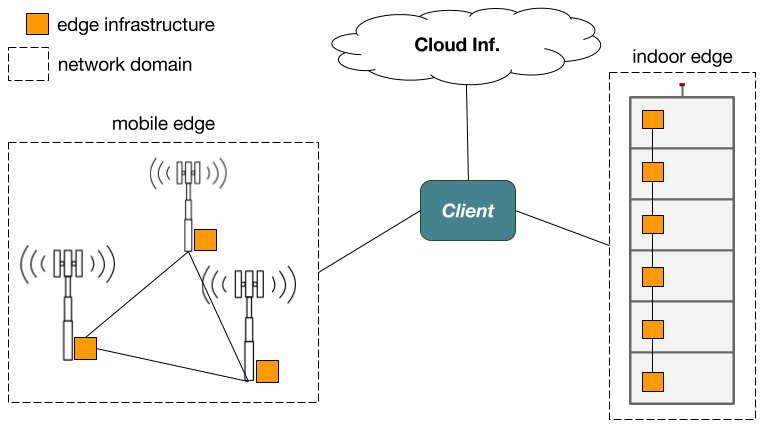
\includegraphics[width=0.51\textwidth]{figs/edge-heterogeneity.png}}
%	\captionsetup[subfigure]{width=0.43\textwidth}	
%	\hfill
%	\subfloat[The heterogeneity of different cloud and edge compute platforms and infrastructures abstracted as domains\label{fig:edge-domain-client}] {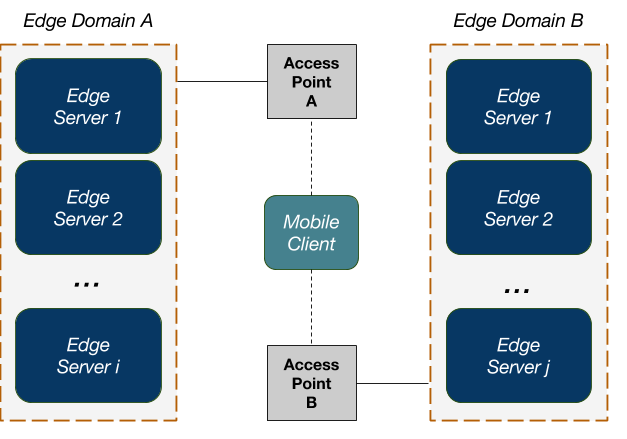
\includegraphics[width=0.43\textwidth]{figs/edge-domain-client.png}}
%	\hfill\null
%	\caption{Continuum heterogeneity}\label{fig:1}
%\end{figure}

%In addition, different kinds of edge infrastructure (e.g., more powerful servers or single board computers) or the same kind of edge infrastructure at different contexts (e.g., the number of clients in an area is too high in one region and low in another) may fit better with different policies for edge resources usage. 

%Client applications heterogeneity
%Client applications may significantly differ in terms of the QoS they require from services and providers. For example, connected vehicles (CV) may eventually rely on edge services for low-latency computation. A CV entering a given region for the first time is unlikely to be waiting until the edge servers covering that region become ready for providing the service the vehicle requires. Conversely, users of an augmented reality application could eventually wait for a setup time whenever the nearby edge \textit{domain}
%%
%~\footnote{From this point on, the term \textit{domain} is used to abstract whatever computational resources can be employed by different computing platforms (i.e., those used by cloud, mobile-edge, local-edge, and local). It is also implied that edge domains are accessible by clients through some (network) access point (Fig.~\ref{fig:edge-domain-client}).} 
%%
%is not ready. 
%%In both cases, low-latency is an important requirement. However, the later type of application could afford a setup delay which the first could not.
%Accordingly, the unified model should enable the co-existence of applications requiring different QoS levels (\stepcounter{req_count}\textbf{R\arabic{req_count}}); and the priority of the usage of computational resources from resource-constrained domains must be in accordance with the application category and its QoS requirements (\stepcounter{req_count}\textbf{R\arabic{req_count}}).

\subsubsection*{Efficiency}\label{sec:efficiency}

\stepcounter{req_count}

In cloud computing, the infrastructure responsible for hosting and performing services is abstracted away from client applications through virtualization and more recently containerization technologies. In particular, the horizontal scalability provided by virtually unlimited cloud resources enables the optimization of cloud services availability by allowing elastic services to remain accessible and operational independently of the number of requests. Such a high availability suits well the services covering either large or dense areas in which requests are always expected. In contrast, the fine grained nature of edge computing suggests the need of a different approach for the usage of its computational resources~\cite{GarrigaMendonca2017}.

%The elasticity of cloud datacenters is enabled by its horizontal scalability, in which virtual machines or containers can be instantiated in new virtually unlimited physical resources. 


%...in which backend applications are deployed to virtual machines and/or containers....

%A direct replication of cloud computing IaaS model with edge computing infrastructure would not be possible. 

First, because it is unlikely that a significant number of applications could be simultaneously hosted by edge servers using technologies such as virtualization and containerization. Even if containers can be allocated faster than virtual machines~\cite{Quatrocchi2016discrete}, at its best, a minimum amount of resources still needs to be allocated to always-deployed containers. Thus, the scalability of edge computing in terms of number of simultaneous services and clients would be reduced. Second, because it is unlikely that clients of services covering small areas shall always be present. 
To improve efficiency and scalability, the allocation of runtime resources to different services should be opportunistic and without minimum preallocation, unless justified otherwise. % (Req. \stepcounter{req_sub_count}\textbf{R\arabic{req_count}.\arabic{req_sub_count}}). 
Moreover, the fine-grained distribution of edge computing and its resource limitations also suggests that an a priori installation and deployment to all edge servers would impose unnecessary burden. Even if storage is more abundant and cheaper resource than runtime resources like CPU and memory, a proactive and indiscriminate acquisition of service artifacts could compromise the scalability of edge computing. Instead, the acquisition of service artifacts should be opportunistic, unless justified otherwise. % (Req. \stepcounter{req_sub_count}\textbf{R\arabic{req_count}.\arabic{req_sub_count}}).

\subsubsection{Locality \& Context-Awareness}\label{sec:context-awareness}

\stepcounter{req_count}

In a fine grained distribution of edge computing, it is unlikely that different service providers will be able to coordinate and decide which one will serve a given client request. For example, from inside a building with some local edge servers accessible through Wi-Fi direct, a client may still be in contact with other servers accessible through 5G\footnote{Fifth generation of broadband cellular technology}. If both providers host the same services, but are unable to communicate and coordinate the allocation of the client request, it is up to the client to make the decision of which provider to use. Accordingly, clients should have the control over which service providers in the continuum should be used. % (Req. \stepcounter{req_sub_count}\textbf{R\arabic{req_count}.\arabic{req_sub_count}}). 

The discovery of finely distributed edge datacenters is another important aspect to be tackled. Today, networking protocols and technologies are the main responsible for allowing client applications to access cloud services in a transparent way. For this, clients access cloud services by means of well-known Internet names that are resolved by traffic managers and domain-name servers (DNS) technologies. The datacenters hosting cloud services are, at best, coarsely distributed among continents, countries, or broader regions. Conversely, finely distributed edge datacenters may be part of the local network infrastructure (e.g., domestic and office infrastructures). Such configuration requires the discovery of local providers by clients. % (Req. \stepcounter{req_sub_count}\textbf{R\arabic{req_count}.\arabic{req_sub_count}}).


%In these cases, services names are mapped to either the servers hosting them or to intermediate components (e.g., traffic managers) responsible for transparently routing client requests to datacenters covering their area. 
%In contrast, in a , a similar transparency may not be possible. 



%Additionally, to allow services to be opportunistically deployed based on the awareness of clients in their coverage area, clients must advertise their requirements to service providers (Req. \stepcounter{req_sub_count}\textbf{R\arabic{req_count}.\arabic{req_sub_count}}).

%clients must be aware of alternative domains (Req. \stepcounter{req_sub_count}\textbf{R\arabic{req_count}.\arabic{req_sub_count}}); and 

%First, because 

%Second, because clients can switch from one network to the other at their discretion or make simultaneous use of different connections.

%Additionally, as mobile clients can enter or exit a given area, their connectivity with a given edge domain may be lost. The less time a mobile client remains connected to a domain, the lower the chances of loosing connection before it is still processing that client's request. Thus, if services are not currently available in one domain, the later should not proxy the request to another domain. Instead, clients should perform direct requests to the cloud instead of having their request forwarded by the edge domain itself.

%In particular, two scenarios of edge computing are possible: 1) edge servers are part of the telecommunications infrastructure (e.g., they are located at cellular base stations); 2) edge servers are part of conventional infrastructure  (e.g., they are located at malls, concert halls, stadiums, office buildings, parks, etc). 
%
%In the first kind of scenario, which correspond to MEC, networking technology could be employed to make the decision of using edge or cloud infrastructure transparent for the client. For instance, active components at the base stations could divert the traffic coming from clients connected to that base station to local edge servers whenever the requested services are available or to the cloud otherwise~\cite{MEC_ROUTING}. 
%
%Analogously, the second kind of scenario would require local network infrastructure components like access points and routers to actively divert the traffic from clients to edge servers in that location upon availability or to the cloud otherwise.
%
%In both cases, clients requests would be transparently handled by either edge or cloud servers, with infrastructure components responsible for taking the edge-or-cloud decision. However, in the event of both types of edge infrastructure to coexist, the client would have to participate of an edge-or-edge kind of decision.


%For instance, at a given moment, the  client device may decide to switch from the mobile-edge domain to the local-edge domain. 

%As such, whereas independent edge servers would not see each other, the client would be able to see them and decide which one suits it the best.

%In addition to the client participation in a edge-or-edge kind of decision, there is an argument in favor of giving the client also the responsibility for the edge-or-cloud type of decision: mobility. 


%\begin{figure}[tbp]
%	\centering
%	\captionsetup[subfigure]{width=0.5\textwidth}	
%	\null\hfill
%	\subfloat[Heterogeneus and indpendent types of edge domains (mobile and indoor) in range of communication with a client device\label{fig:edge-heterogeneity}]{ 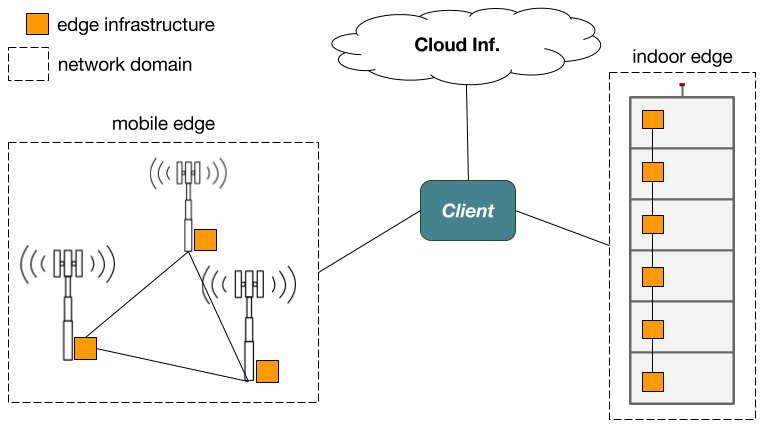
\includegraphics[width=0.5\textwidth]{figs/edge-heterogeneity.png}}
%	\captionsetup[subfigure]{width=0.45\textwidth}	
%	\hfill
%	\subfloat[In the case no edge service is available, client performs direct requests to the cloud and eliminate the dependency with intermediary edge domain infrastructure\label{fig:domain-selection}] {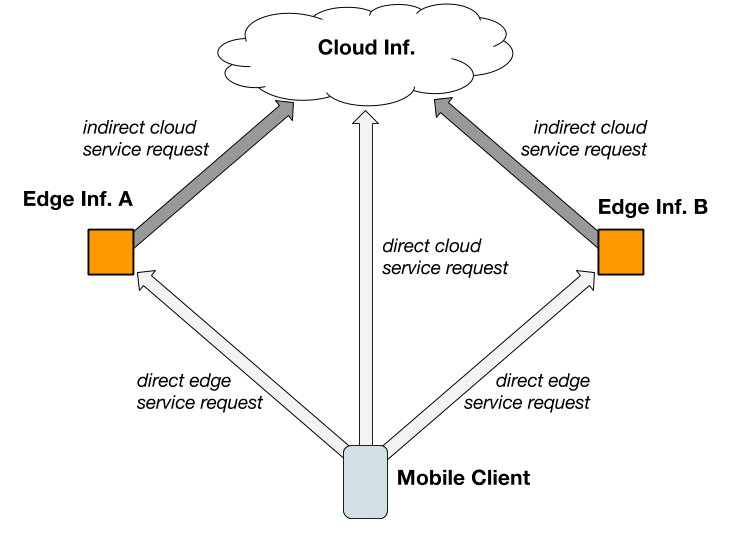
\includegraphics[width=0.45\textwidth]{figs/domain-selection.png}}
%	\hfill\null
%	\caption{Edge heterogeneity and client awareness}\label{fig:no-label-here}
%\end{figure}

%TODO: replace R2 with: Control over forwarding from edge to cloud. Soft vs. strong constraint. Soft = I can also run on cloud if needed. Strong = Never go to cloud.
	
\subsubsection{Automation and Encapsulation}

\stepcounter{req_count}

Last but not least, the multiplicity of finely distributed edge datacenters implies not only a limitation in terms of availability of resources, but also a large scale of servers to be managed. Such characteristic motivates the automation of the operational aspects of services life-cycle for two reasons: 1) to avoid the burden and costs of manual operation of a large scale of finely distributed servers; and 2) to allow service life-cycle to be efficiently managed. Whereas the later aspect is addressed by the serverless computing paradigm and the FaaS execution model, a complete self-management of services life-cycle is still missing.

%Automation is also needed to allow services to be seamlessly displaced from different parts of the continuum. Accordingly, automation should encompass the operational aspects of services life-cycle, including resource allocation for different services 
%(Req. \stepcounter{req_sub_count}\textbf{R\arabic{req_count}.\arabic{req_sub_count}}) 
%and their installation. 
%(Req. \stepcounter{req_sub_count}\textbf{R\arabic{req_count}.\arabic{req_sub_count}}). 
%Finally, automation should also encompass the choice of alternative services by a client. %(Req. \stepcounter{req_sub_count}\textbf{R\arabic{req_count}.\arabic{req_sub_count}}).


%in the context of a shared platform 

%Following a serverless architecture, the application developer has control over the code they deploy into the infrastructure. 
%The model should be automated and transparent, where the developer is unaware of which infrastructure is using to run her applications. 

%In specific, the allocated resources should be scaled to zero where no servers are actually running when the application's function code is not used, and there is no cost to the user nor overload to the platform.


%Therefore, the management of computational resources must be automated and not depend on  manual intervention from human administrators (\textbf{R\arabic{req_count}}).


%Differently from classical \textit{on-premise} servers, edge should benefit from the automation and other characteristics of the A3-E model. As a result, local-edge servers can be seen as automated black boxes requiring no manual maintenance.	
	
%The fulfillment of the above requirements would leverage the potential of edge computing by optimizing the usage of its resources and consequently allowing a larger number of client applications to share the costs of edge infrastructure. Moreover, the resulting unified model would work as an extension of today's cloud IaaS/FaaS with the twofold purpose of enabling applications with low-latency requirements to rely on edge domains and to augment the computational power of mobile devices through mobile-to-edge computation offloading. Last but not least, the computing power of highly available and elastic cloud services would remain as an essential part of the continuum.

\subsection{Example Scenario}

\begin{figure}[tbp]
	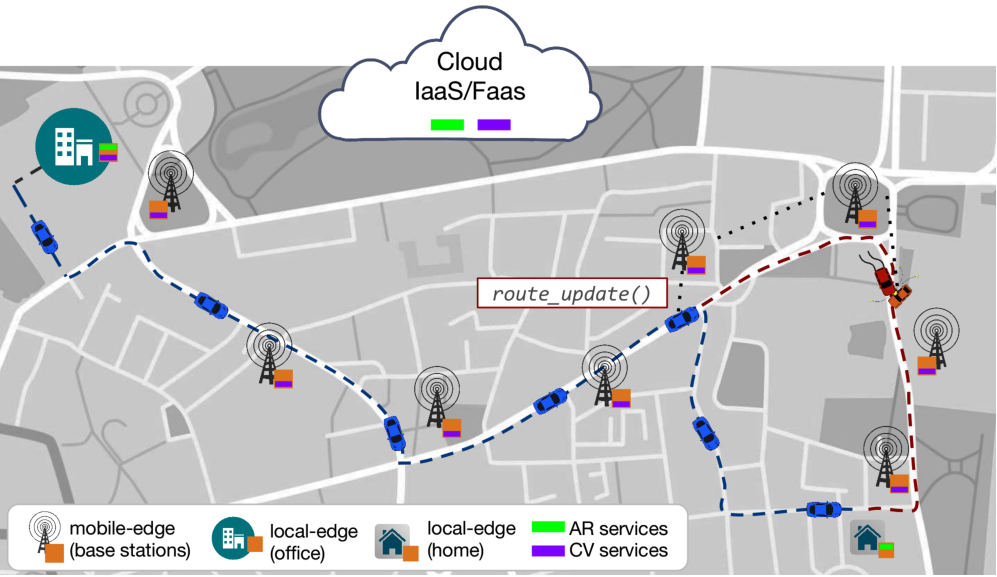
\includegraphics[width=0.8\textwidth]{figs/Continuum-Scenario}
	\caption{Heterogeneous applications such as Augmented Reality (AR) and Autonomous Vehicles (AV) interact with services deployed along the computational continuum (cloud, mobile-edge, local-edge, and mobile)}
	\label{fig:continuum-scenario}
\end{figure}

%Throughout this section an example scenario (Fig.~\ref{fig:continuum-scenario}) is used to illustrate the use of A3-E model and the cloud-edge-mobile continuum with different applications employed by a person with visual impairment.
We illustrate the computational continuum in an example scenario  that starts in a user's office and finishes in his home and involves different applications that rely on services executed in the cloud, edge, or in the user's own devices. 
First, let us assume the existence of a local edge server in the user's office (hereafter called \textit{local-edge}). This server is owned by the company to extend the computational capabilities of devices operated by its employees. In our example, the user makes use of an %Augmented Reality (AR) application that parses objects from scenes captured from his mobile device camera and produces audible information. The application involves two heavyweight tasks: the image processing from the captured scenes ($IP$); and the text-to-speech ($TTS$).
Augmented Reality (AR) application to craft three dimensional virtual objects added to his desk table. In specific, this application involves heavyweight image processing from the captured scenes. By offloading this task to the local-edge, the user is exempt from recharging her glasses and can improve productivity. 

After work, our user leaves his office and enters his Autonomous Vehicle (AV). During its way home, the vehicle will make use of edge services deployed at servers located at cellular base stations (hereafter called \textit{mobile-edge}) to receive low-latency updates about the best plan to reach its destination. Within milliseconds, the vehicle is suggested to make a turn just in time to avoid the traffic formed by an accident a few blocks ahead. In particular, the new path consists of residential streets without coverage of mobile-edge services. The AV continues to fetch updates, this time from cloud services. The additional network latency is compensated with the low speed limit of the residential area.

Already at home, the user's smartphone gets in reach of communication with the local-edge server owned by him. In that day, he finds out about a new mobile game application 
%for visually impaired users
. Upon installation, the edge server becomes aware of a new edge-compliant application and, meanwhile the app is already running locally, proceeds with the setup of required services. Once available, the client application becomes aware of these services and switches from local to edge with the purpose of preserving the smartphone's resources. Not only the game performance improves, but also the battery consumption is reduced.  

In the scenario described above, different parts of the continuum have been employed by user's devices. Whilst edge services were privileged, cloud services remain fundamental, as edge domains were not always available. Furthermore, the edge services consumed by the AR application and those consumed by the AV were pre-allocated by the office's local-edge and the mobile-edge services. In contrast, an AR application was able to make use of local resources from a mobile device until edge services were opportunistically made available by the local-edge server at user's home.

%services for which network latency is not disruptive are in the cloud (e.g., persistence, stateful components, and large part of the business logic).



\subsection{A3-E Phases}

\begin{figure}[tbp]
	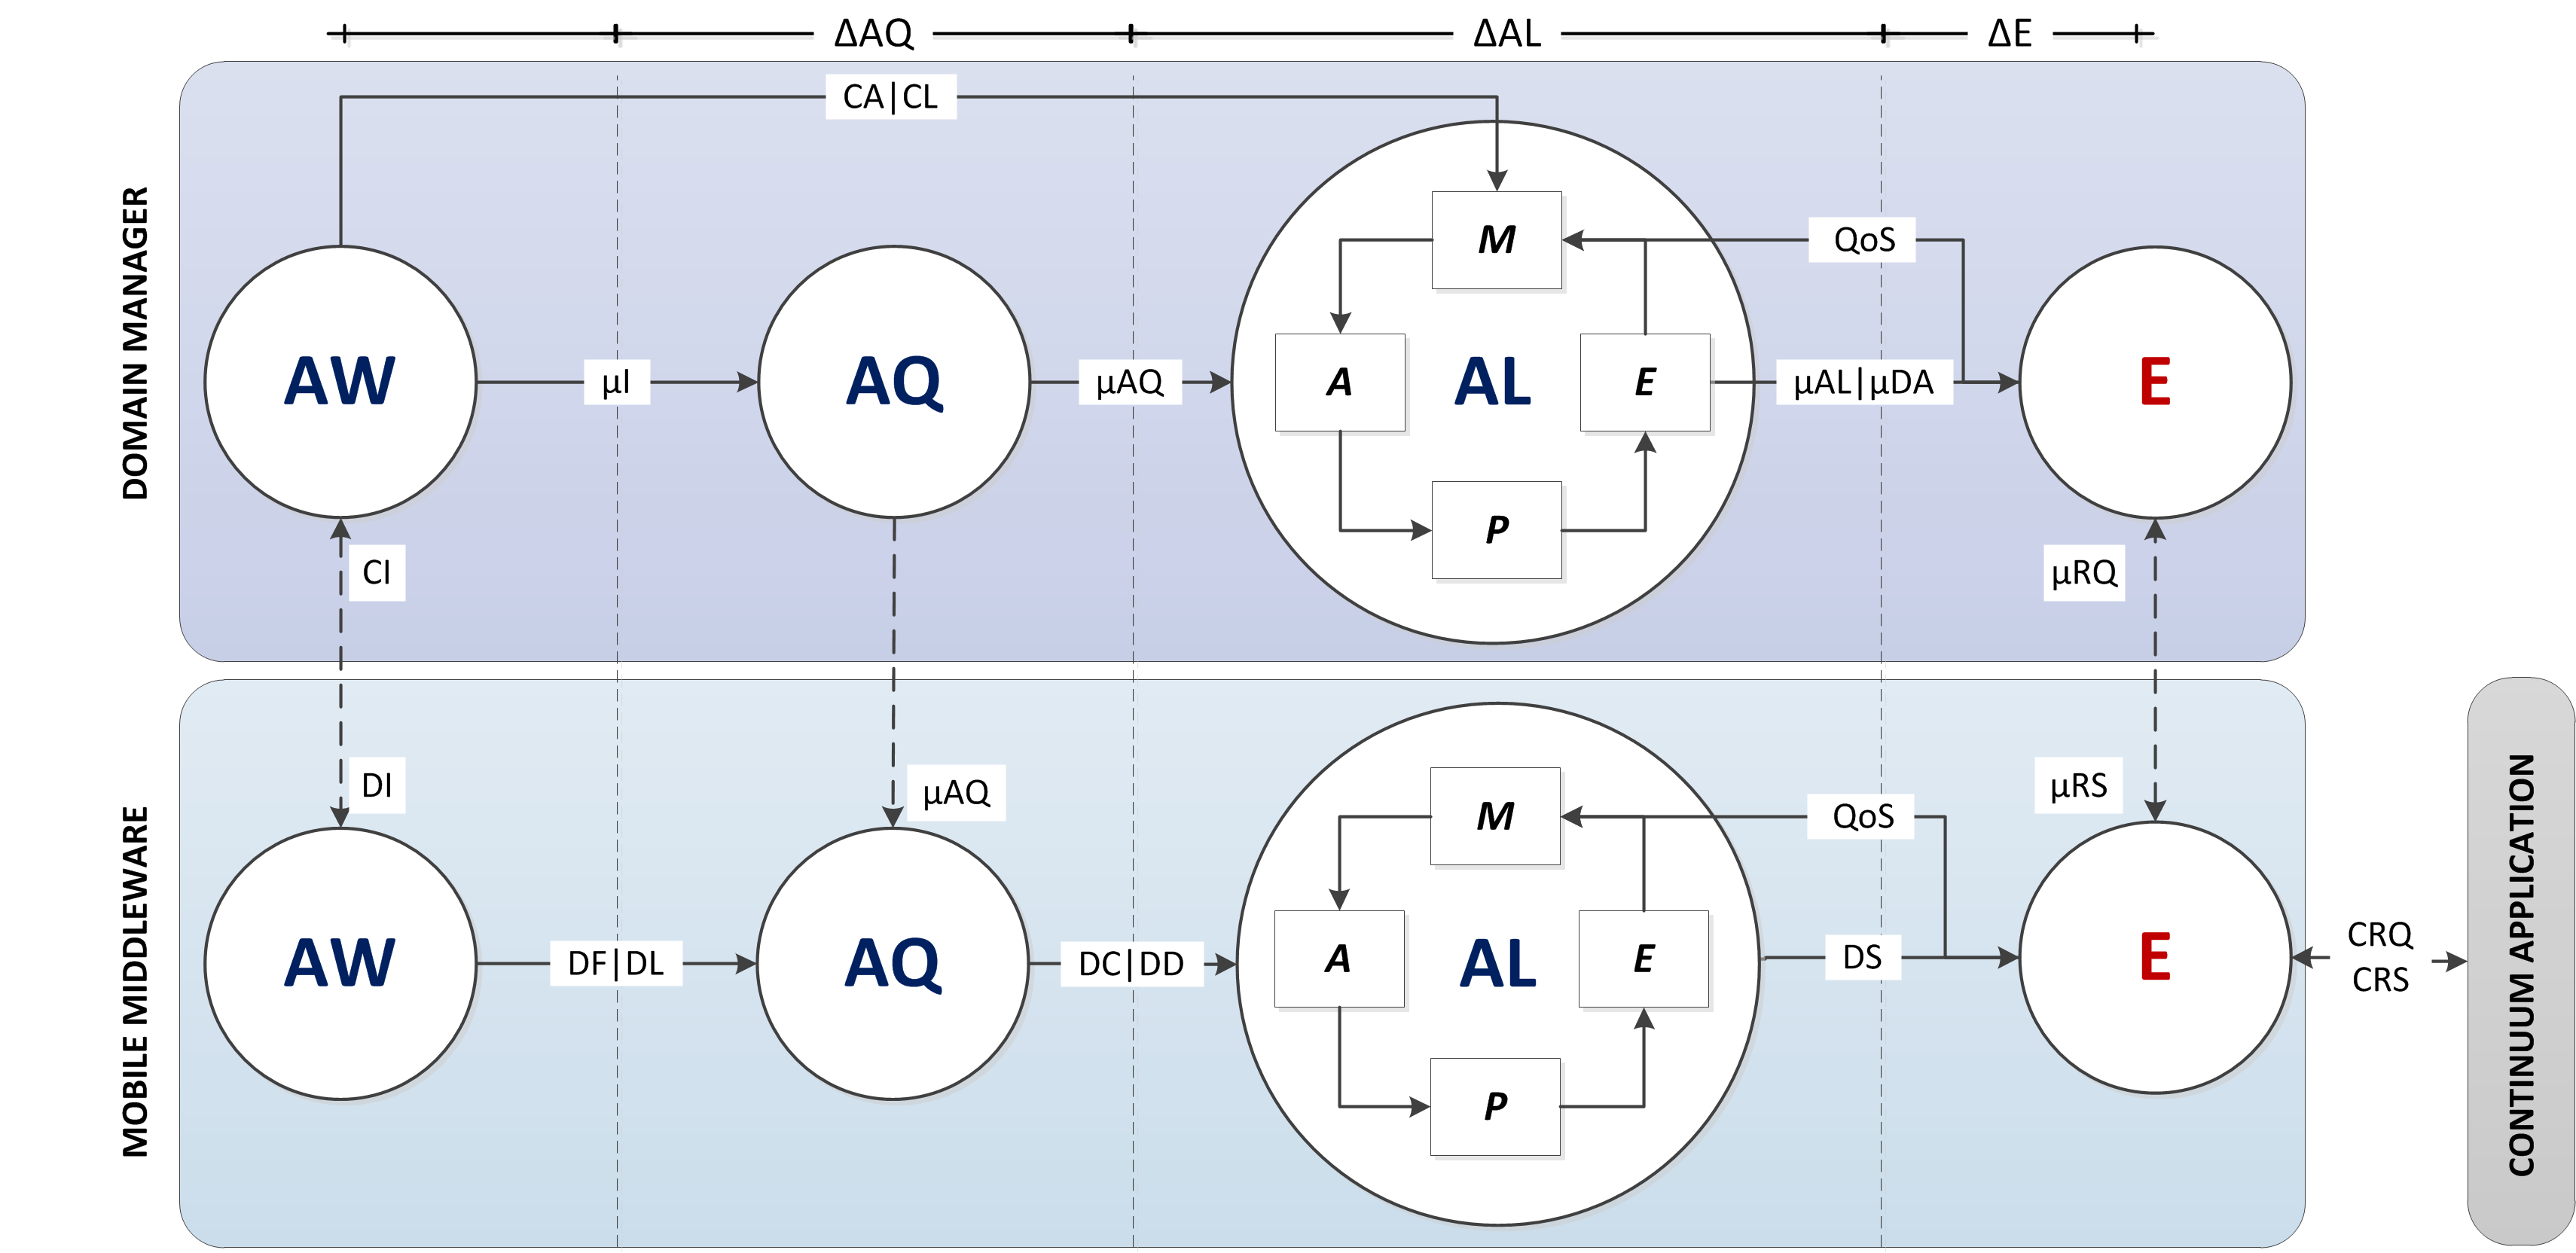
\includegraphics[width=0.9\textwidth]{figs/A3-E.png}
	\caption{Different phases of the A3-E model; phases are delimited by vertical lines and the main activity of each phase by the label within each phase; labels within parenthesis represent the states of a domain (client) with respect to a client (domain)}
	\label{fig:A3-E-model}
\end{figure}

The A3-E provisioning model consists of four phases: \textit{(\textbf{A}wareness), (\textbf{A})cquisition, (\textbf{A})llocation, and (\textbf{E})ngagement}. Each of these phases encompasses activities that take care of specific concerns in the interaction among clients and different types of server infrastructure. 

%A3-E addresses all actors in the computational continuum formed by mobile devices, edge, and cloud servers. 

A3-E model is flexible with respect to its constituting phases and addresses all the constituents of the computational continuum. In specific, the diagram in Fig.~\ref{fig:A3-E-model} represents the scenario in which an edge domain first contacts an application hosted by a mobile client. This instance of the A3-E model is used to illustrate the use of all four phases in the model. 

Next, the four A3-E phases are further described and mapped to the requirements elicited in  Section~\ref{sec:requirements}. Later on, other possible instances of the A3-E model are correlated with scenarios of the computational continuum.

\subsubsection{Awareness Phase}\label{sec:A3-E-awareness}

%Why do we need awareness?
%CA: awareness is not needed because the edge domain should always be coupled to the network infrastructure; network components shoudl aways route traffic to existing edge servers; additionally, the edge domain should be able to acquire and allocate services upon detection of the first requests.  
%A: A3-E model is agnostic w.r.t. the use of network technologies to route traffic to the edge servers; a given domain my count on network components to traffic route to its servers instead of negociating directly with clients aware of its existance; nonetheless, the lack of awareness limits the acquisition and deployment of services to reactive, as the domain would only identify a given service upon the first request has been made. Clients, in the other hand, would not be able to choose from alternative domains. 

In A3-E, the Awareness phase has the following purposes:

\begin{itemize}
	
	\item To enable a domain to pro-actively initialize other phases (namely acquisition and allocation) based on its awareness about client applications hosted by clients in the domain coverage area (Requirement Rx);
	
	\item To enable clients to choose from alternative domains based on their awareness about these domains (Requirements Ry); 
	
\end{itemize}

Thus, from the domain side, the lack of (client) awareness prevents the triggering of the acquisition and subsequently allocation phases based on the detection of a client. From the client side, the lack of (domain) awareness prevents clients of deciding which alternative domains must be used. 

\subsubsection{Acquisition Phase}\label{sec:A3-E-acquisition}

In its turn, the Acquisition phase has the following purposes:

\begin{itemize}

	\item To enable a domain to pro-actively download assets used by services that must become available in that domain (Requirement Rx);
	
	\item To enable clients to pro-actively identify their requirements (services) and allow the domain to pro-actively download them (Requirement Rx);

\end{itemize}

From the domain side, the lack of acquisition implies that service assets must be previously made available. Nonetheless, the preliminary acquisition of a large number of assets is limited by the domain storage capability. 

Conversely, the automated and opportunistic acquisition of service assets improves storage efficiency with the cost of a setup time $\Delta_AQ$. For instance, domains that become aware of clients' requirements may pro-actively start the acquisition phase and become ready for allocation before the first service request arrives.

%otherwise, domains must rely on the detection of a first service request or some other triggering condition to start the acquisition phase and, after setup time $\Delta_A$, become ready for allocation. 

\subsubsection{Allocation Phase}\label{sec:A3-E-allocation}

The allocation phase addresses has the following purposes:

\begin{itemize}

\item To enable the automated process of making a service ready for execution through the allocation of computational resources (Requirement Rx); and

\item To enable clients to choose among different alternative domains that may happen to be available (Requirement Ry).

\end{itemize}
 
Cloud providers already implement automated scaling mechanisms, e.g, with the allocation of virtual machines and container instances on demand. More recently, the FaaS model introduced zero-allocation mechanism, in which stateless functions may remain deallocated until they are invoked (cold start). Once the demand increases, the FaaS platform may respond with additional instances of the required functions.

From the domain side, A3-E adheres to the dynamic allocation of computational resources for services execution. Applications that can not afford the delay (hereafter named $\Delta_{AL}$) of a cold start must rely on services that are always kept available with minimum allocation. Instead, whenever cold start is acceptable, the zero-allocation provides a more efficient usage of computational resources.

From the client-side, once the awareness phase has been active and identified the current alternative domains, the client may consider QoS values from each domain to make the decision of which one to engage. Conversely, the lack of awareness implies that client engagement with a specific domain must be solved by means of a well-known name. In the later case, networking traffic components are responsible for routing client requests to specific domains.

\subsubsection{Engagement Phase}\label{sec:A3-E-engagement}

Finally, the \textit{engagement} phase models the interaction between a client and a service. At this stage, the requested service must be already acquired and allocated for execution. 

\subsection{Phase Transitions and Policies}

The A3-E model is also flexible with respect to the transitions among subsequent phases. In particular, distinct policies may define different transition behaviors. Figures~\ref{fig:A3-E-domain} and~\ref{fig:A3-E-client} depict, respectively, the possible transitions among states of a domain with respect to a client application and vice-versa. Each state is mapped to the corresponding phase in Fig.~\ref{fig:A3-E-model}.

\begin{figure}[tbp]
	\raggedright
	\subfloat[Different states of a given edge domain with respect to a given client application; the transitions between states triggered by domain events are guarded by policies that may vary according to the type of edge infrastructure and application\label{fig:A3-E-domain}] {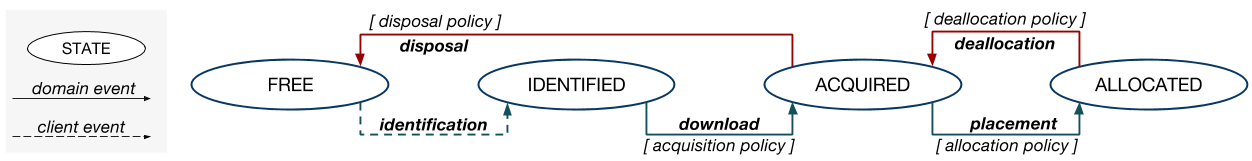
\includegraphics[width=0.95\textwidth]{figs/A3-E-domain.png}}\hfill
	
	\subfloat[Different states of a given client with respect to a given edge domain; the transitions between states triggered by client events are guarded by policies that may vary according to the client requirements\label{fig:A3-E-client}] {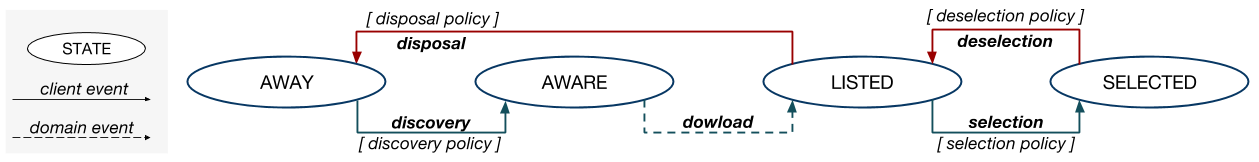
\includegraphics[width=0.95\textwidth]{figs/A3-E-client.png}}\hfill
	\caption{States and transitions among A3-E phases} \label{fig:A3-E-states}
\end{figure}

The use of a specific policy may depend on factors like:

\begin{itemize}

\item The type of domain (e.g., cloud, mobile-edge, local-edge); and

\item The type of application and the SLA among clients and service  providers;

\end{itemize}

Above all, the choice of a policy is affected by two conflicting properties: 1) the efficiency of domain resource usage (domain side); and 2) the application tolerance for service setup delay (client side). Eq.~\ref{eq:setup_delay} models the total delay of service setup.

%\Delta_{NET} + 
\begin{equation}\label{eq:setup_delay}
L_{SETUP} = \Delta_{AW} + \Delta_{AQ} + \Delta_{AL};
\end{equation}

The first term represents the time it takes for clients and domains to become aware of each other. The second term represents the time for downloading all assets of a specific service, whilst the last term represents the time for allocating resources for the service execution. 

Considering the first request from a client application as the reference event, the more \textit{reactive} the policies are to that event, the less time domain resources are likely to remain idle before it happens. Conversely, the more \textit{pro-actively} services are made ready for execution, the less delay the first request to each of these services are served with. 

%\subsubsection{Acquisition Policies}

The \textit{acquisition policies} in Fig.~\ref{fig:A3-E-domain} can be:

\begin{itemize}

\item \textbf{P}roactive: acquisition phase starts upon external event preceding the arrival of the first request (e.g., the prediction of service usage); first request is not delayed by $\Delta_{AQ}$;

\item \textbf{S}equential: acquisition phase starts as soon as awareness phase finishes; first request may be delayed by $\Delta_{AQ}$; or

\item \textbf{R}eactive: acquisition phase starts as soon as the first request for a service arrives (frozen start); first request may be delayed by $\Delta_{AQ}$.

\end{itemize}

%\subsubsection{Allocation Policies}

The \textit{allocation policies} in Fig.~\ref{fig:A3-E-domain} can be:

\begin{itemize}

\item \textbf{P}roactive: allocation phase starts upon external event preceding the arrival of the first request (e.g., triggered by a prediction of service usage); first request is not delayed by $\Delta_{AL}$;

\item \textbf{S}equential: allocation phase starts as soon as acquisition phase finishes; first request may be delayed by $\Delta_{AL}$; or

\item \textbf{R}eactive: allocation phase starts as soon as the first request for a service arrives; first request may be delayed by $\Delta_{AL}$ (also known as cold start).

\end{itemize}

%In the opposite direction, both \textit{deallocation} and \textit{disposal policies} can either be:
%
%\begin{itemize}
%
%\item Proactive: deallocation/disposal is triggered upon external event (e.g., triggered by a prediction of ); ; 
%
%\item Reactive: allocation phase starts as soon as the first request for a service arrives (cold start).
%
%\end{itemize}


%The client must either have opted for that specific domain during allocation phase or, in case of awareness/allocation has not been employed by the client, it must rely on external components to route its request to a given domain in a transparent way.

%the start of the allocation phase may be triggered by the end of the acquisition phase, or it may be combined with additional conditions required for the allocation phase to start.
%
%For instance, the awareness of a client application, which may happen pro-actively through the awareness phase, may be the additional condition for the allocation phase to start. In this case, allocation may finish before the first request to arrive, eliminating the delay of a cold start.
%
%For instance, a client would engage with a cloud service by firing a request to a well-known Internet name. At some point of the network infrastructure (e.g., at the cellular base station), a component diverges the request to the edge servers in that domain.
%
%In contrast, a local-edge domains may advertise its existence to clients in connection range. Each client, upon awareness of multiple domains (in this case, the edge and the cloud), decides which domain to use. If the client QoS requirement is network latency, the decision should favor the local-edge. 


%The acquisition-allocation transition, in its turn, is modelled by two alternative policies: 
%
%\begin{itemize}
%
%\item proactive allocation: phase starts as soon as acquisition phase finishes; or
%
%\item reactive allocation: phase starts as soon as acquisition phase finishes and the client notifies its intention for using that domain.
%
%\end{itemize}
%
%Finally, reverse transitions are single and dependent on the specific policies for deallocating and disposing of application assets. 
%In accordance with Requirement R6, the aforementioned policies are useful for different classes of applications, as well as different types of edge computing infrastructure and different usage contexts.
%
%


%\subsection{A3-E Instances}\label{sec:A3-E-instances}

\begin{center}
\begin{table}[htbp]
\small
\caption{Different instances of the A3-E model and  corresponding policies}\label{tab:A3-E-instances}
\begin{tabular}{ r c c c c }
\toprule

& \textbf{A}WARENESS & \textbf{A}CQUISITION	& \textbf{A}LLOCATION 	& \textbf{E}NGAGEMENT  	\\

\midrule

IaaS-Cloud		& DNS	& OFFLINE				& HOT-START		& BY REQUEST\\
FaaS-Cloud	& DNS	& OFFLINE				& COLD-START	& BY REQUEST\\						
FaaS-Edge	& A\&D	& [P, S, R]				& [P, S, R]		& BY REQUEST\\	
FaaS-Edge	& DNS	& [P, R]				& [P, S, R] 	& BY REQUEST\\

\bottomrule
\end{tabular}
\end{table}
\end{center}
\normalsize

%Later in this section, it will be explained how both mobile and cloud alternatives are considered by the \textit{selection} activity of the client's allocation phase.

%Thus, whereas the \textit{engagement} phase represents the core of the interaction between clients and servers and the \textit{allocation} phase is already part of today's cloud computing, the additional phases of \textit{acquisition} and \textit{awareness} address the particularities of different types of edge computing.

Table~\ref{tab:A3-E-instances} correlates the possible instances of the A3-E model with different scenarios of the cloud-edge-mobile continuum and the policies that may be adopted. The policy adopted by a phase affects which policies may be adopted by the subsequent phase (e.g., a reactive acquisition implies a reactive allocation, as service assets must first be acquired before been deployed, whilst a proactive acquisition may be combined with a reactive allocation). The possible instances in Table~\ref{tab:A3-E-instances} are:

--- \textbf{IaaS-Cloud}: services hosted in the cloud are, in most of the cases, reachable by means of a well-known Internet name (therefore, no dynamic awareness is employed). Assets used by these services are preliminarily deployed to cloud servers (thus, no dynamic acquisition is employed). Virtual machines and containers are pre-allocated (hot start), and cloud's elasticity mechanisms take care of the (de)allocation of resources according to a service level agreement (SLA). Finally, cloud services are invoked by clients (engagement phase). 

--- \textbf{FaaS-Cloud}: the FaaS model distinguishes from the cloud instance described above by enforcing the use of stateless functions that can be quickly allocated for execution without minimum pre-allocation (cold start).

--- \textbf{FaaS-Edge}: services hosted in the edge, in contrast, may need to opportunistically advertise their existence (awareness phase), acquire application assets (acquisition phase), make them ready for invocation (allocation phase), before finally been able to expose the required computation as services to be consumed. Such opportunistic modality of edge computing, nonetheless, may co-exist with others in which: 1) services are transparently accessed through well-known Internet names; 2) service assets are pre-acquired (offline acquisition); and 3) services are pre-allocated in order to increase the readiness required by certain types of applications (hot start). 

\subsection{A3-E: Reference Architecture}\label{sec:a3-e-reference-architecture}

\begin{figure}
  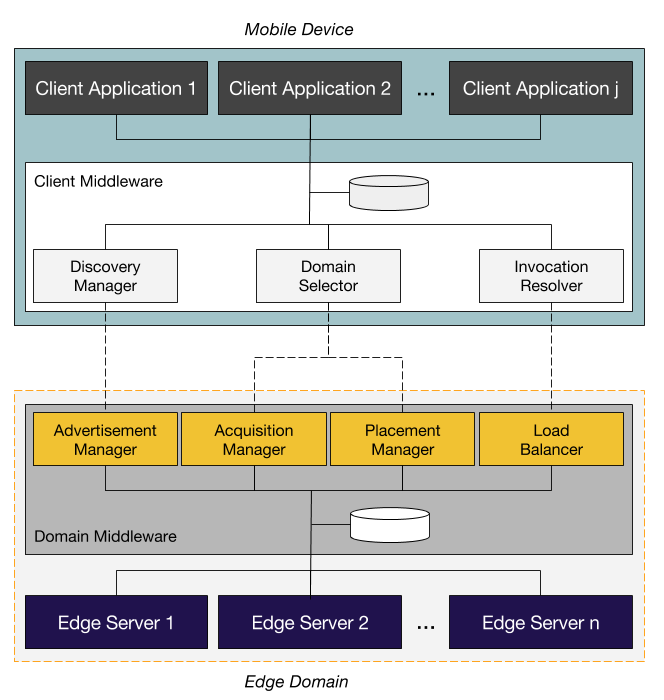
\includegraphics[width=0.6\textwidth]{figs/reference-architecture.png}
  \caption{TODO}
  \label{fig:reference-architecture}
\end{figure}

\begin{figure}
	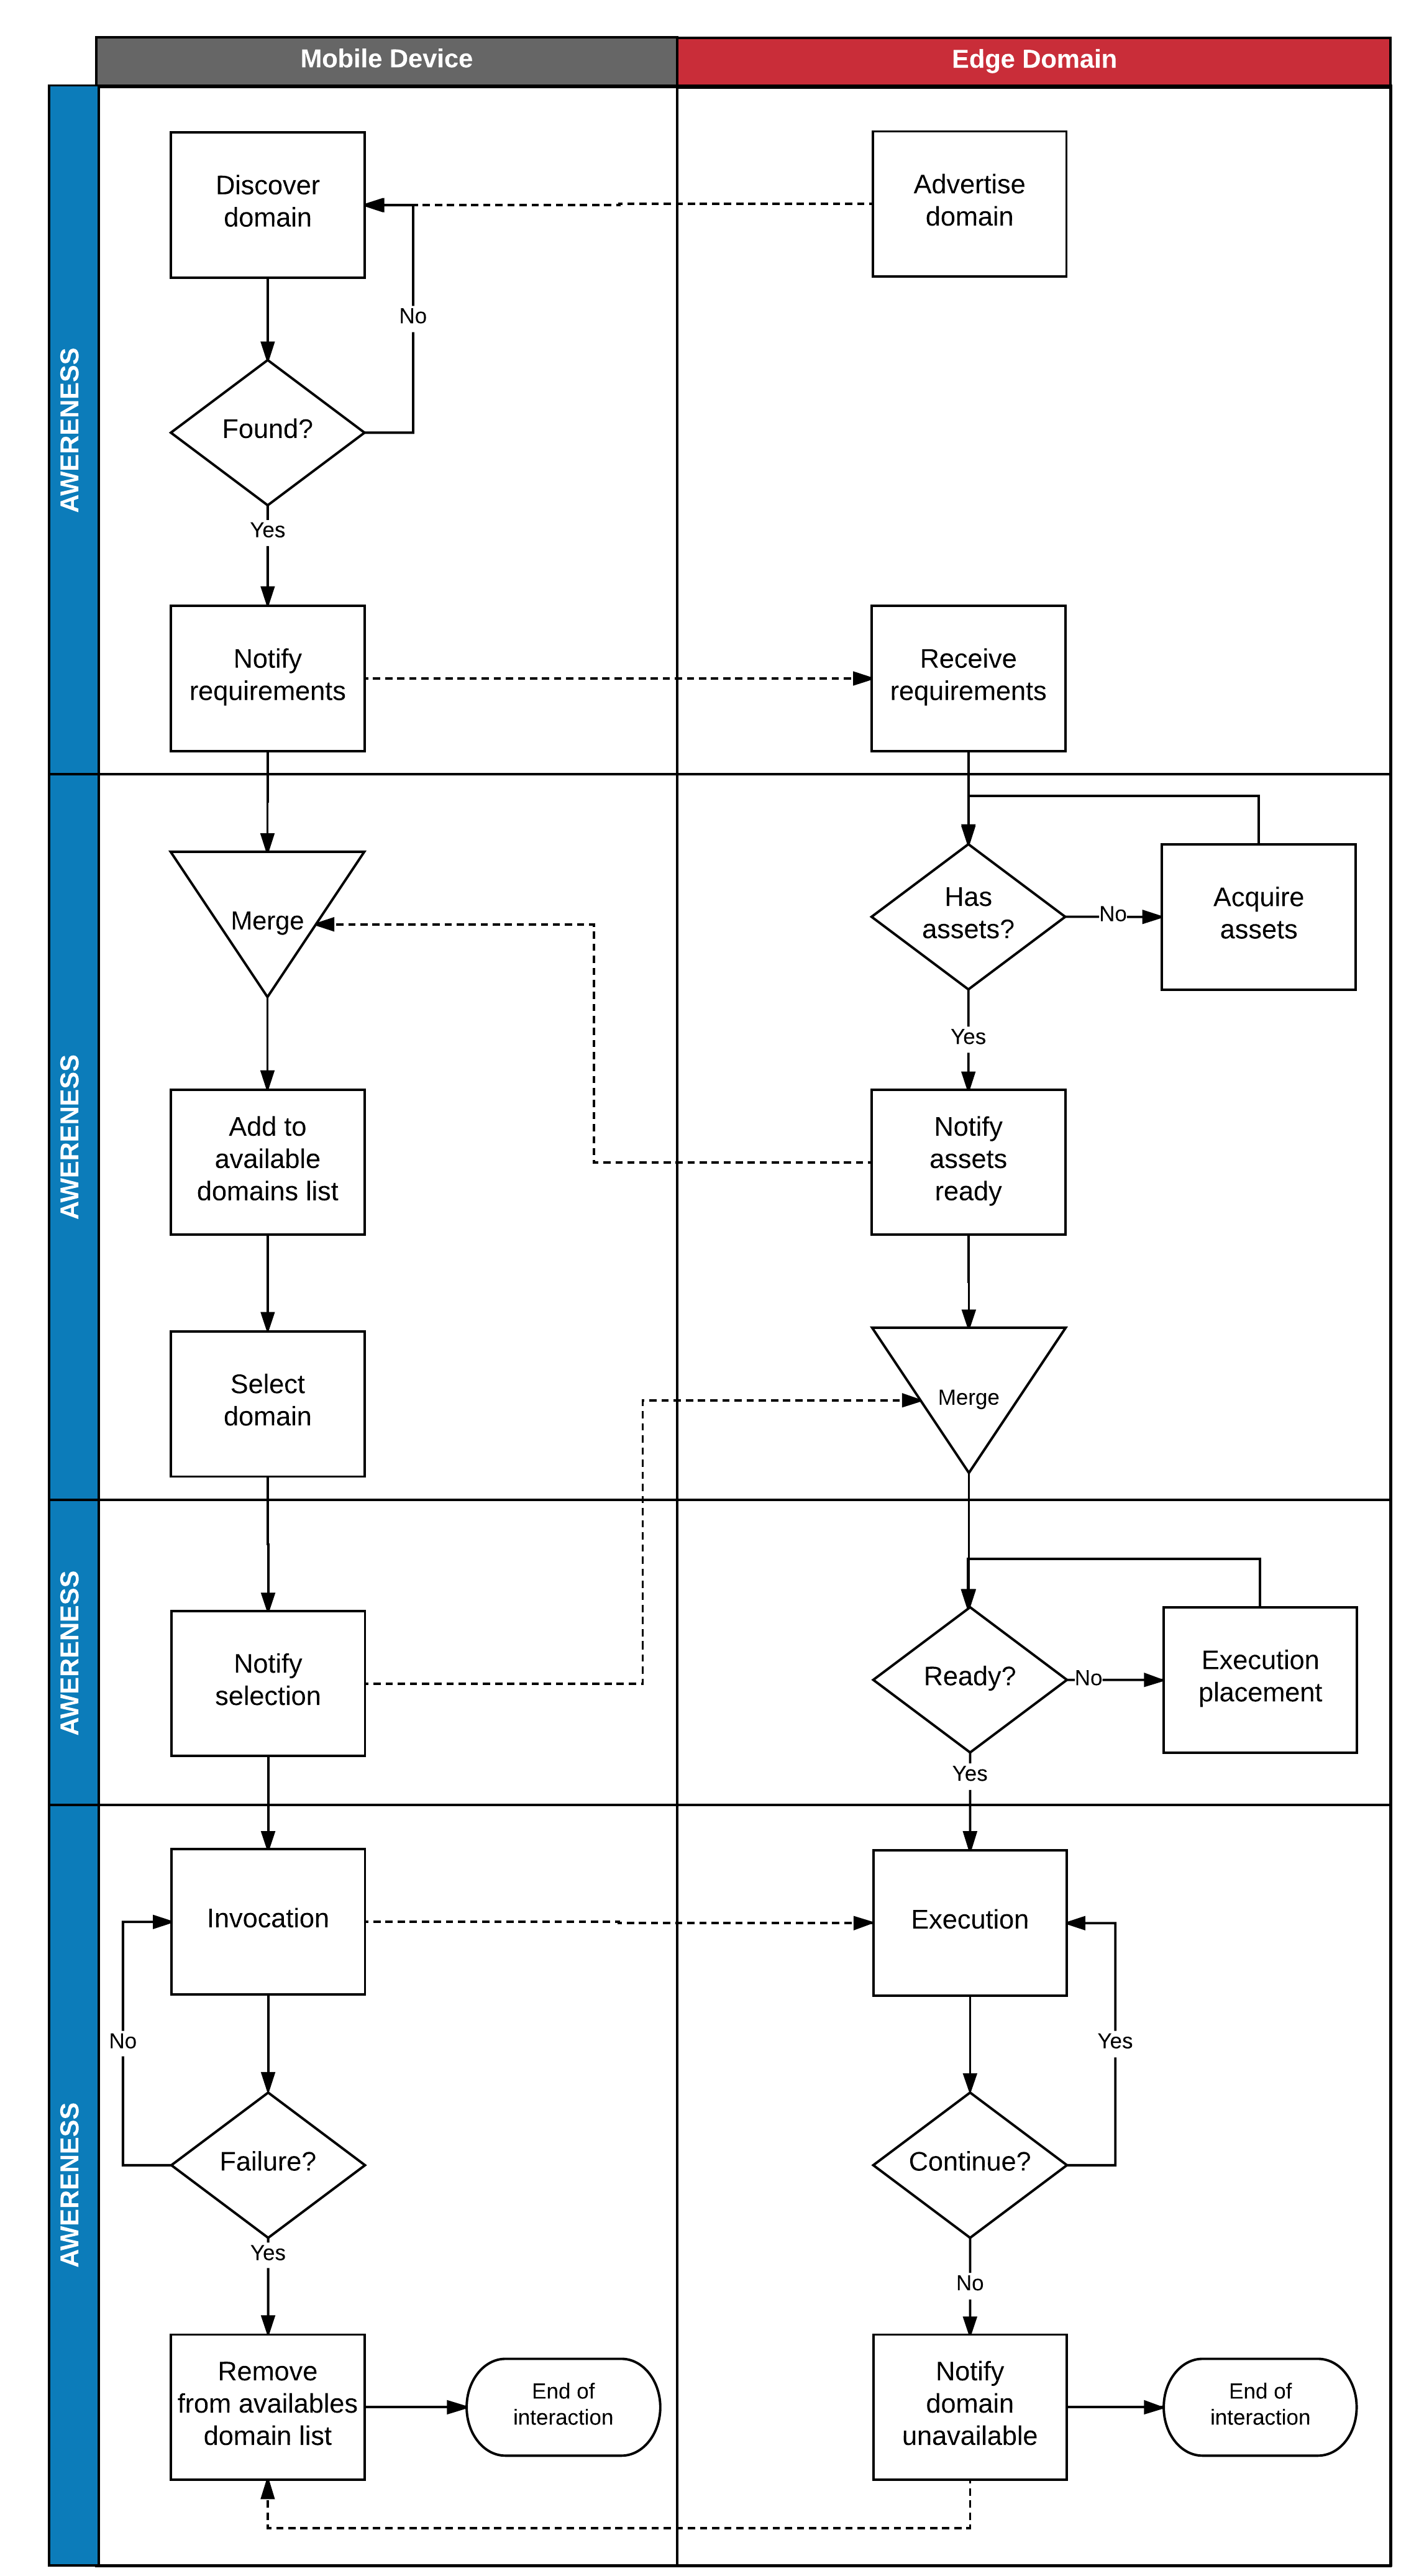
\includegraphics[height=\textheight]{figs/activities.png}
	\caption{TODO}
	\label{fig:activities}
\end{figure}

TODO: decide whether to leave activity diagram and details about HOW to perform each of the A3-E phases as part of the proposal or the evaluation; 

In accordance with requirement R1, edge domains perform the advertisement of their existence to whatever clients may be in reach. Potential clients, in their turn, must perform the discovery of edge domains. Before a given domain is found, it remains unknown to that client.

To address requirement R3 and R4, edge domains must remain free with respect to some application until the contact with a potential mobile client hosting that application. This condition refers to both the storage of application assets (e.g., code, libraries, etc), as well as the allocation of these assets for execution (e.g., deployment and instantiation of a restful application). 

Once a given domain has been discovered, the client must proceed with the identification of the application it is running. This process enables the edge domain to download whatever assets required by that specific application.  

The acquisition of application components does not make them ready to be executed. Instead, valuable resources like memory and CPU are kept free w.r.t. this application until the domain proceed with the placement of the application components as part of the allocation phase. The later activity corresponds to the allocation of resources from one or more domain servers required for the application execution. 	

Finally, once the allocation phase is finished, the domain is ready to perform the computation required by the application. For instance, following a request-response protocol, clients can fire requisitions to that domain. These activities are part of the engagement phase.

The separation of phases emphasizes not only the different concerns involved, but also the distinction between the moments they occur. The transition among phases may either be sequential, meaning that one phase starts as soon the previous finishes, or conditional, meaning that additional condition(s) must be met before the next phase can start. 	

%the client applications hosted by a mobile devices interact with a domain through a client middleware; the domain has its own middleware responsible for the activities in the A3-E model and interfaces with the servers in that domain


\begin{figure}
  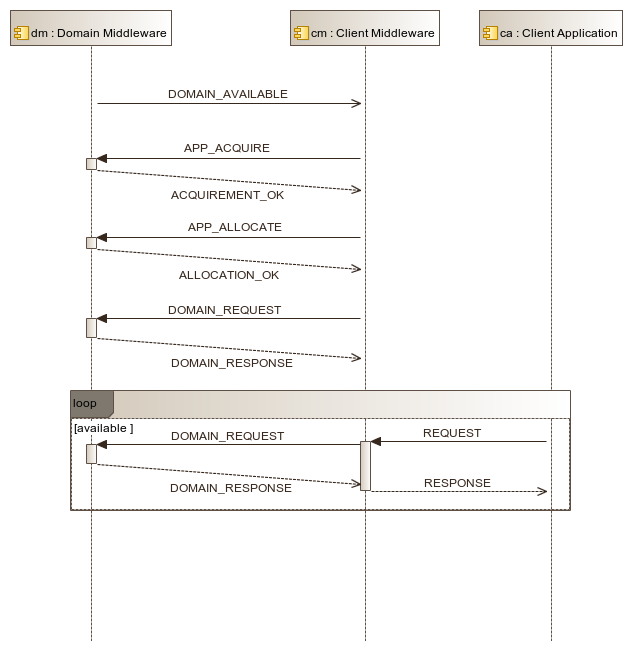
\includegraphics[width=0.6\textwidth]{figs/protocols.png}
  \caption{TODO}
  \label{fig:protocols}
\end{figure}

